%Travail technique
	%But?
	%Overview (Mockups, workflows)
	%Algorithme
	%Architecture et Design
	%Implémentation (langage et librairies utilisés)
	%Utilisation (screenshots, etc)


\chapter{Travail technique}
	\thispagestyle{document}
	
\section{But}
\label{sec:but}
\par Le but est d'utiliser les suites de tests d'un projet comme spécifications de celui-ci. Ces spécifications contiennent deux types de valeurs très importante. Premièrement les variables accessibles lors d'un comportement exécuté par l'application : les entrées. Ensuite la valeur attendu de ce comportement : la sortie. À la manière de Nopol\cite{nopol}, le but est de trouver une relation entre les entrées et la sortie à l'aide de solver SMT. Cette relation représentera le comportement nominal de l'application.

\section{SMT}
\label{sec:smt}
\par Un problème SMT est un problème dit de \textit{satisfiabilité modulo théories}. DEFINIR




\section{Overview}
\label{sec:overview}
\par Premièrement, la phase de collecte de données est effectuée pour obtenir les entrées et la sortie pour chaque tests. Ensuite, cette approche va généré un problème SMT basé sur la même implémentation de Nopol\cite{nopol}. Un solver sera alors appelé pour essayer de résoudre se problème. Si une solution existe, il est nécessaire de transformer la solution en code adéquate afin de générer un patch. Pour finir, les tests seront lancer à nouveau pour verifier la véracité du patch. La figure \ref{fig:workflow} représente le schéma d'exécution de la solution proposé.


\begin{figure}[H]
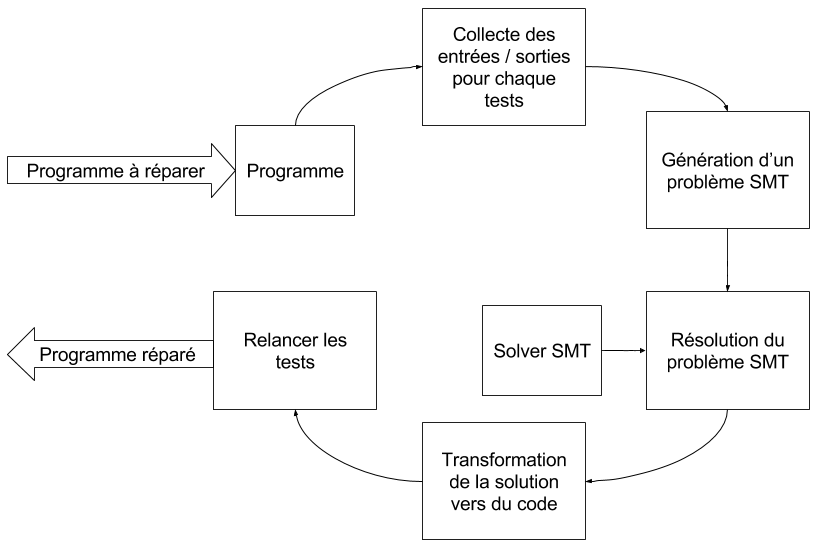
\includegraphics[scale=0.5]{workflowSMT.png}
\caption{Workflow de l'exécution du programme}
\label{fig:workflow}
\end{figure}

\section{Scope}
\label{sec:scope}

\subsection{Programmes}

Programme Java, contenant des tests JUnit défaillant.

\subsection{Forme des tests}

Appel direct de methode dans l'assert

\subsection{Collecte}

Paramètres des méthodes


\subsection{Type des entrées / sorties}

Si tous est entiers/réelles ou boolean, ca marche facilement sinon des problèmes interviennent


\section{Implementation}
\label{sec:implementation}

\par L'implémentation est réalisé en Java. Pour analyser les tests et collecter les entrées / sorties, cette approche utilise Spoon\footnote{\url{http://spoon.gforge.inria.fr/}}, une librairie d'analyse et de transformation de code source.
\par La transformation des spécifications en problème SMT utilise les algorithmes déjà défini dans Nopol\cite{nopol}. Ces algorithmes utilise JSMTLIB\footnote{\url{https://github.com/smtlib/jSMTLIB}}, une librairie permettant la génération de script SMT-LIB\footnote{\url{http://smtlib.cs.uiowa.edu/}}, un langage compréhensible par des solvers SMT.
\par Le solver utilisé est Z3\footnote{\url{https://z3.codeplex.com/}}, ce solver embarque les théories non-linéaires sur les réels, ce qui le démarque des autres.




	

	
		
		
		